\begin{figure}
\setlength{\tabcolsep}{0.5pt}
    \centering
    { \small 
\begin{tabular}{lcccc}
\rotatebox[origin=t]{90}{Original} &
\raisebox{-.42\totalheight}{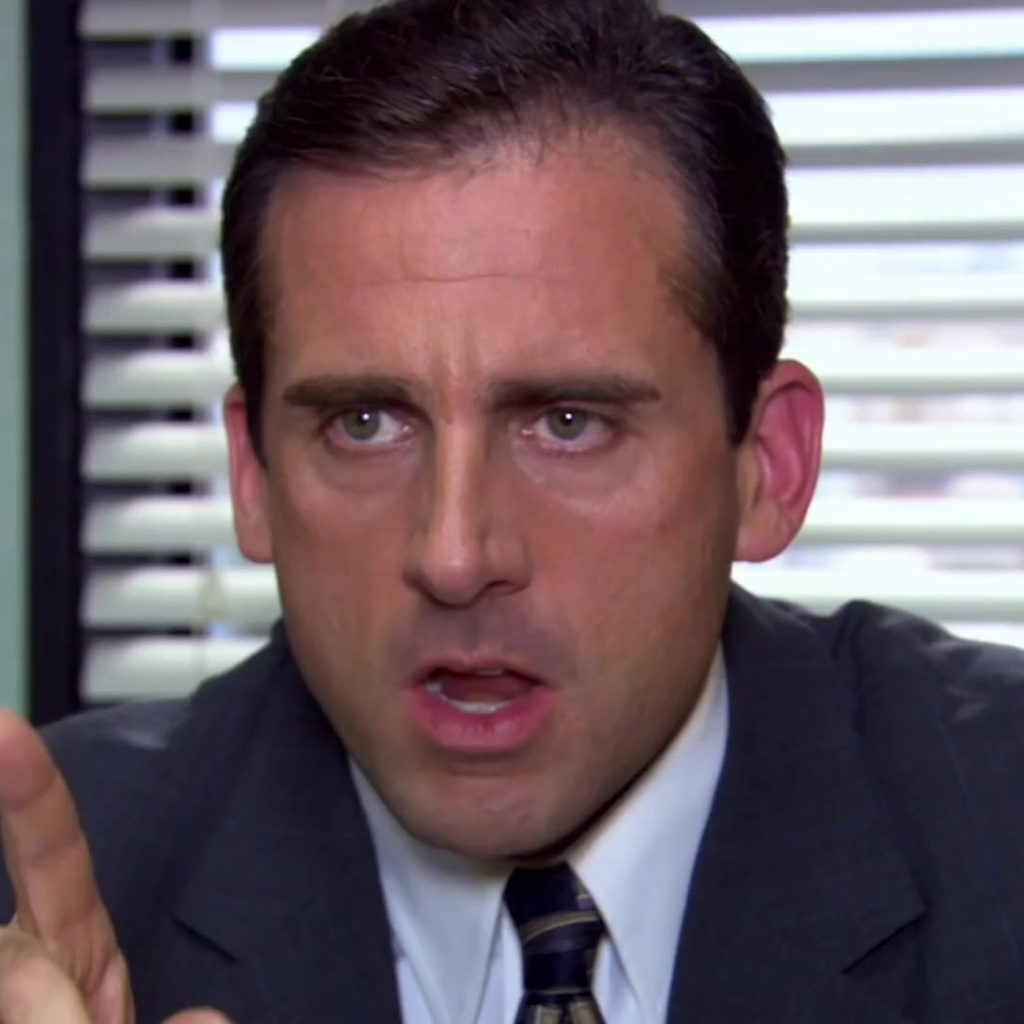
\includegraphics[width=0.24\columnwidth]{resources/images/comparison/original/source_0000.jpeg}} &
\raisebox{-.42\totalheight}{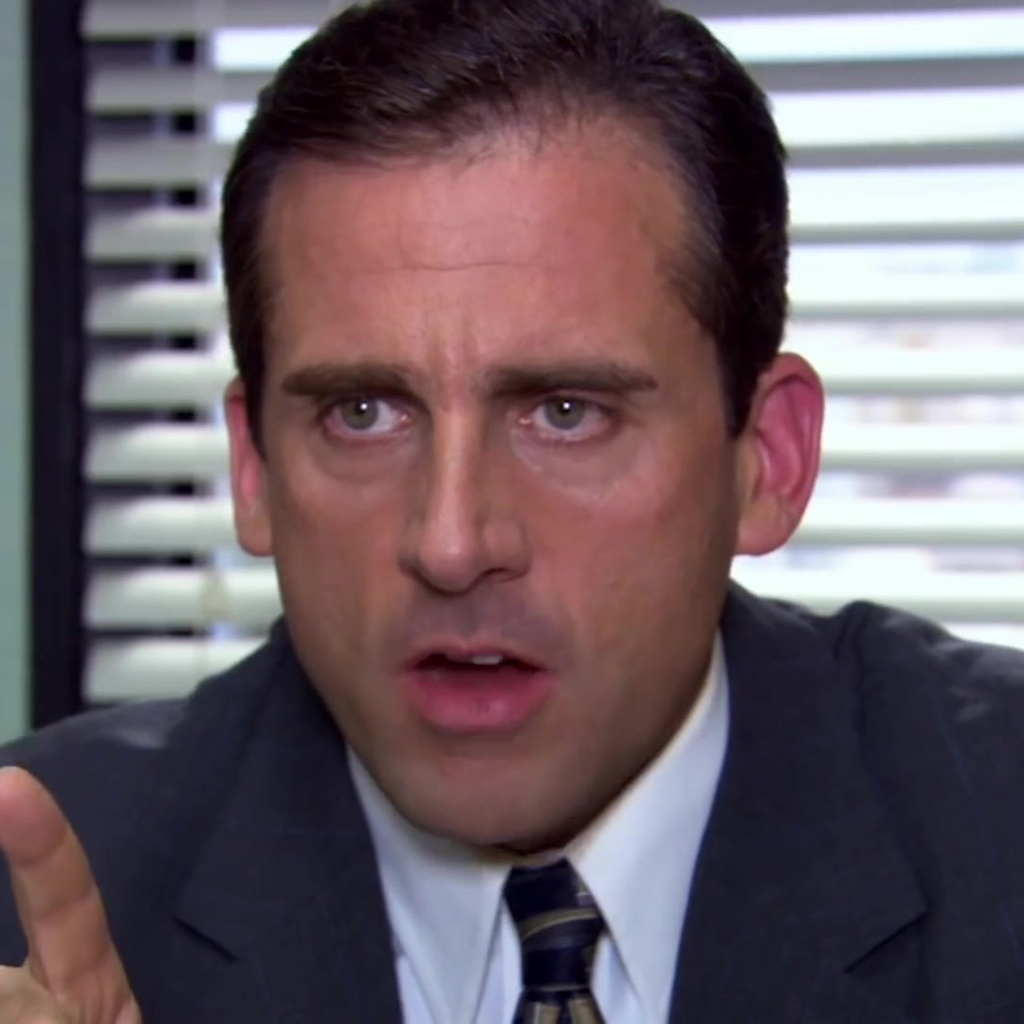
\includegraphics[width=0.24\columnwidth]{resources/images/comparison/original/source_0016.jpeg}} &
\raisebox{-.42\totalheight}{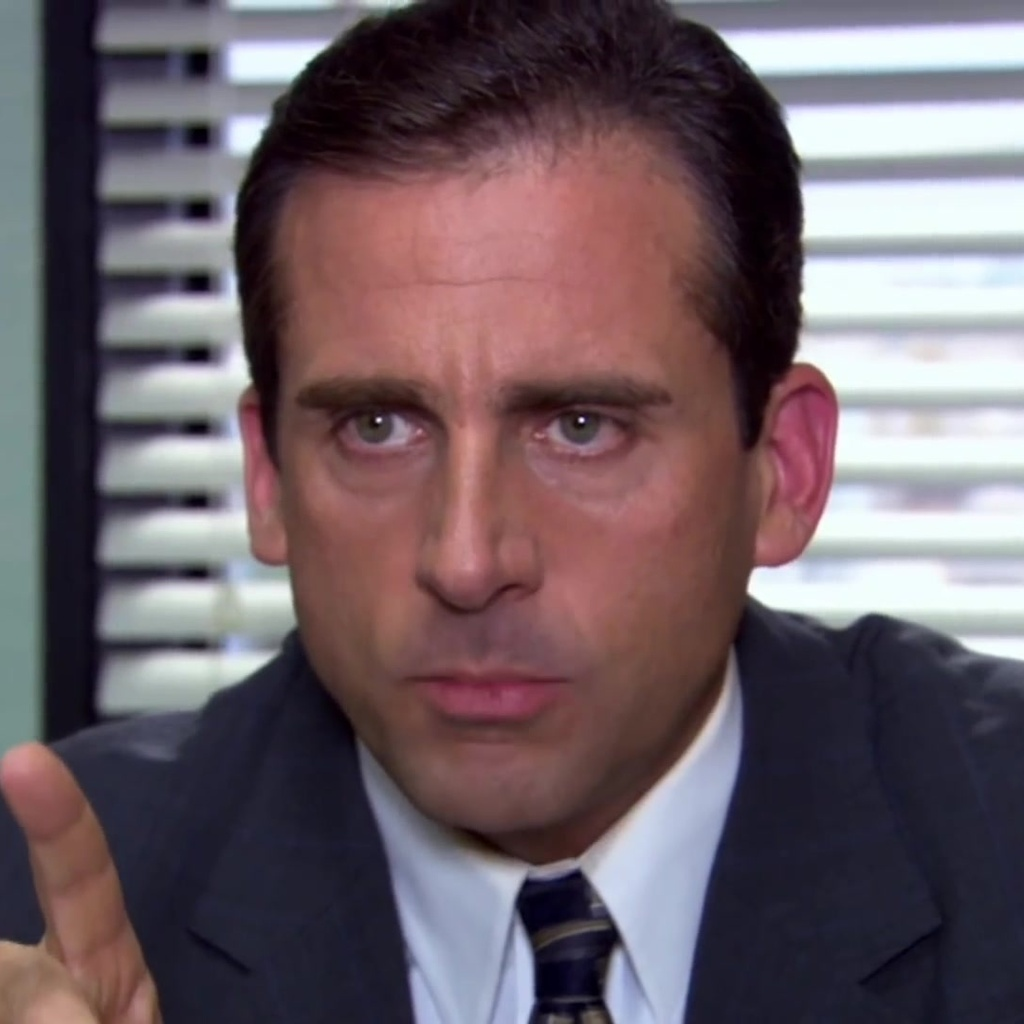
\includegraphics[width=0.24\columnwidth]{resources/images/comparison/original/source_0040.jpeg}} & 
\raisebox{-.42\totalheight}{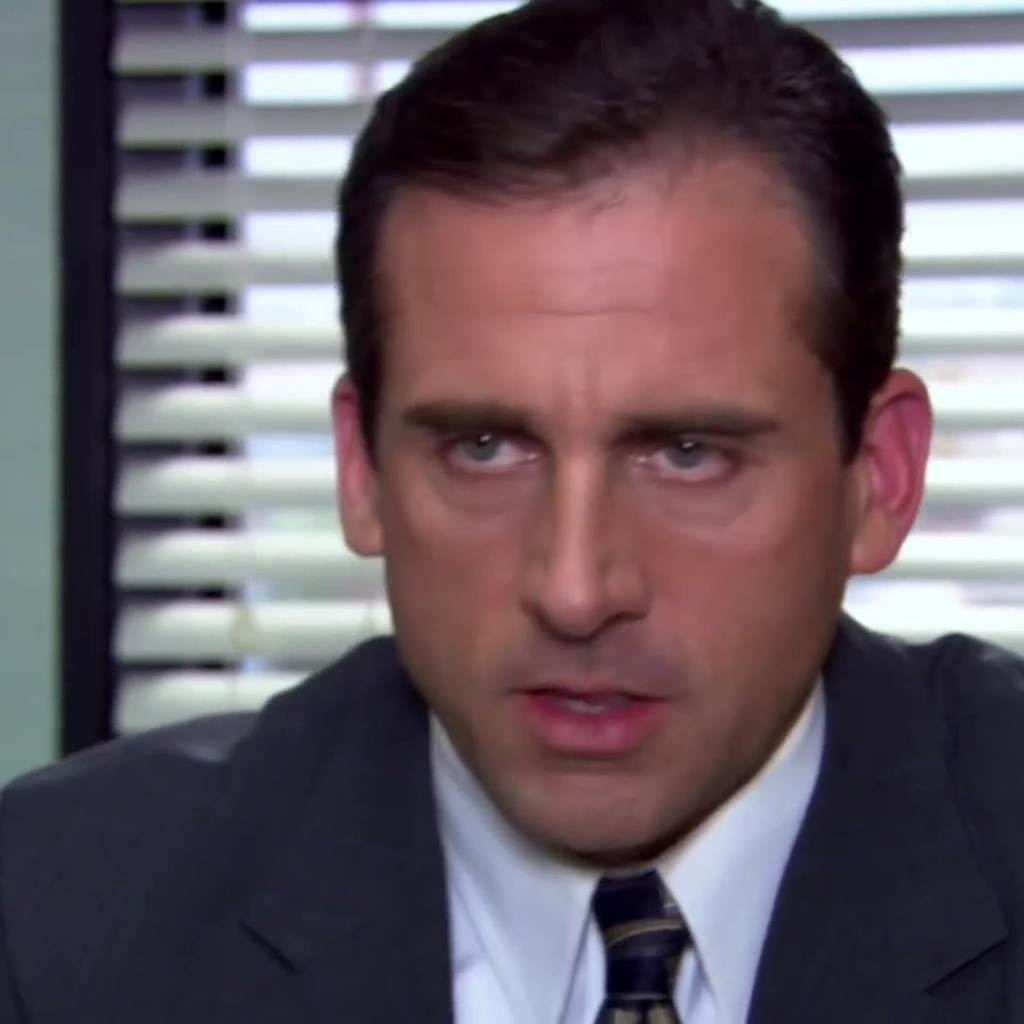
\includegraphics[width=0.24\columnwidth]{resources/images/comparison/original/source_0100.jpeg}} \\
\noalign{\vskip .5mm}
\rotatebox[origin=t]{90}{Yao et al~\cite{yao2021latent}} &
\raisebox{-.42\totalheight}{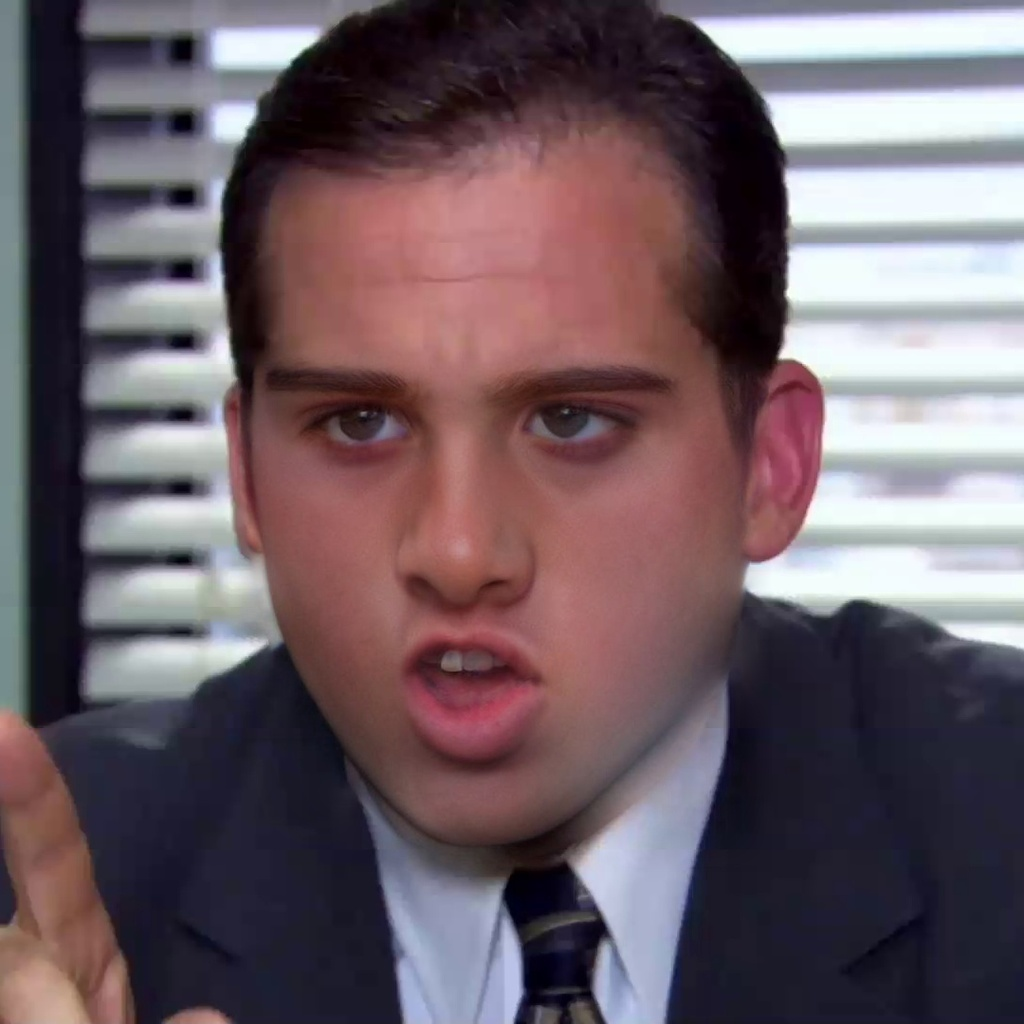
\includegraphics[width=0.24\columnwidth]{resources/images/comparison/latent/frame0000.jpg}} &
\raisebox{-.42\totalheight}{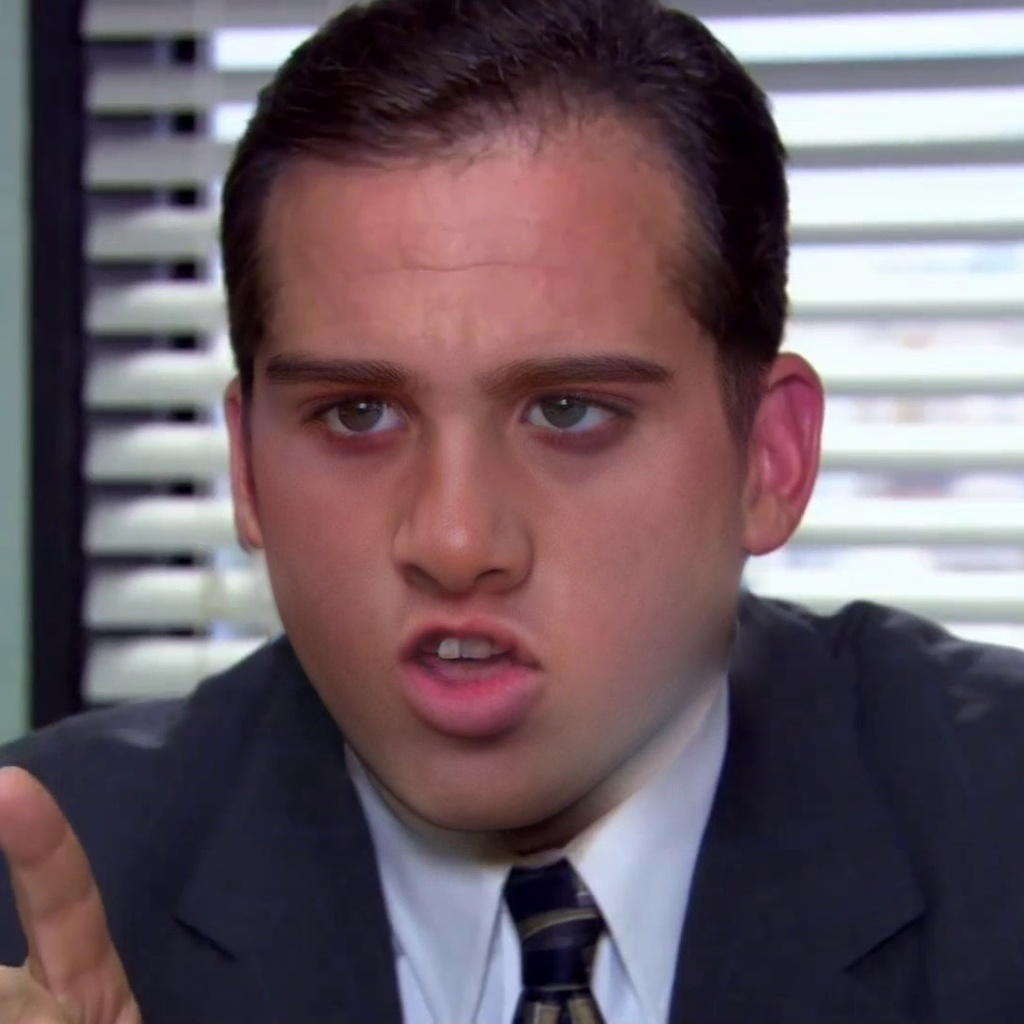
\includegraphics[width=0.24\columnwidth]{resources/images/comparison/latent/frame0016.jpg}} &
\raisebox{-.42\totalheight}{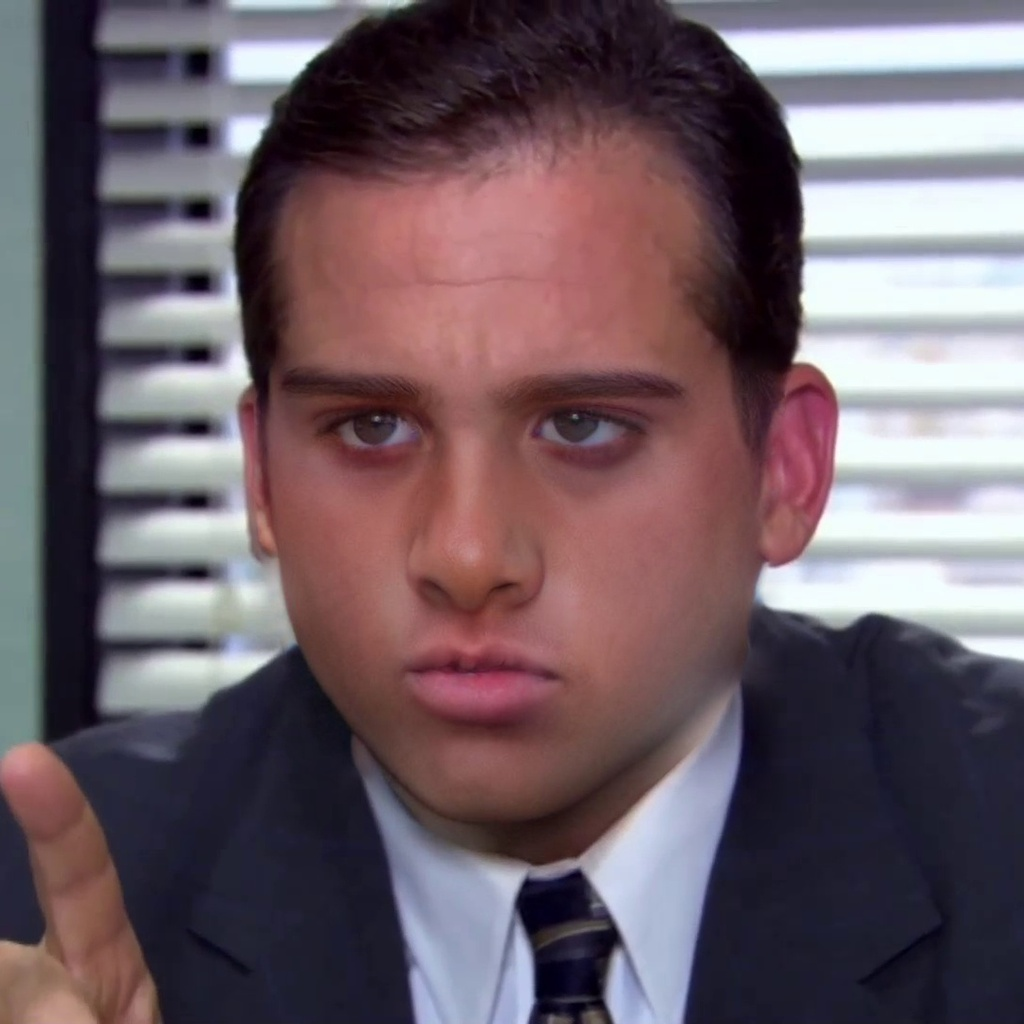
\includegraphics[width=0.24\columnwidth]{resources/images/comparison/latent/frame0040.jpg}} &
\raisebox{-.42\totalheight}{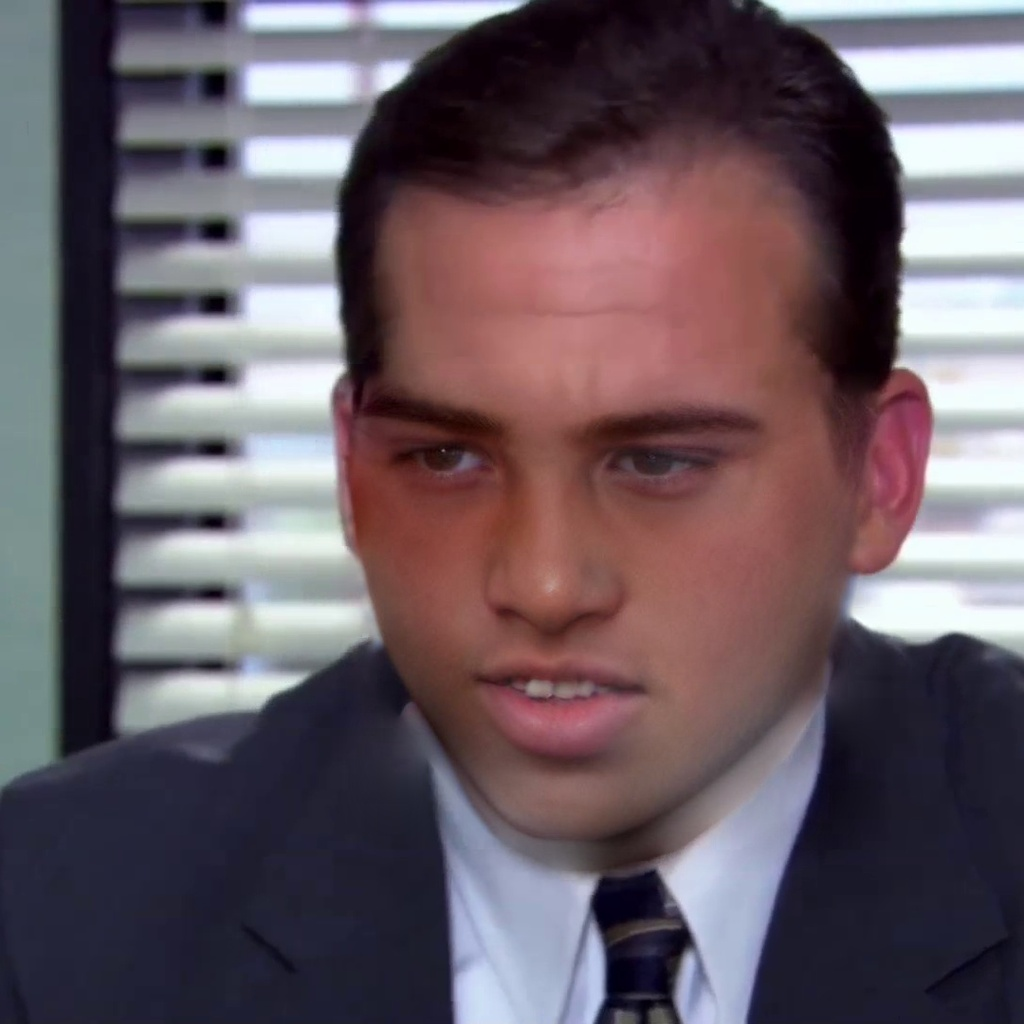
\includegraphics[width=0.24\columnwidth]{resources/images/comparison/latent/frame0100.jpg}}\\
\noalign{\vskip .5mm}
\rotatebox[origin=t]{90}{PTI \shortcite{roich2021pivotal}} &
\raisebox{-.42\totalheight}{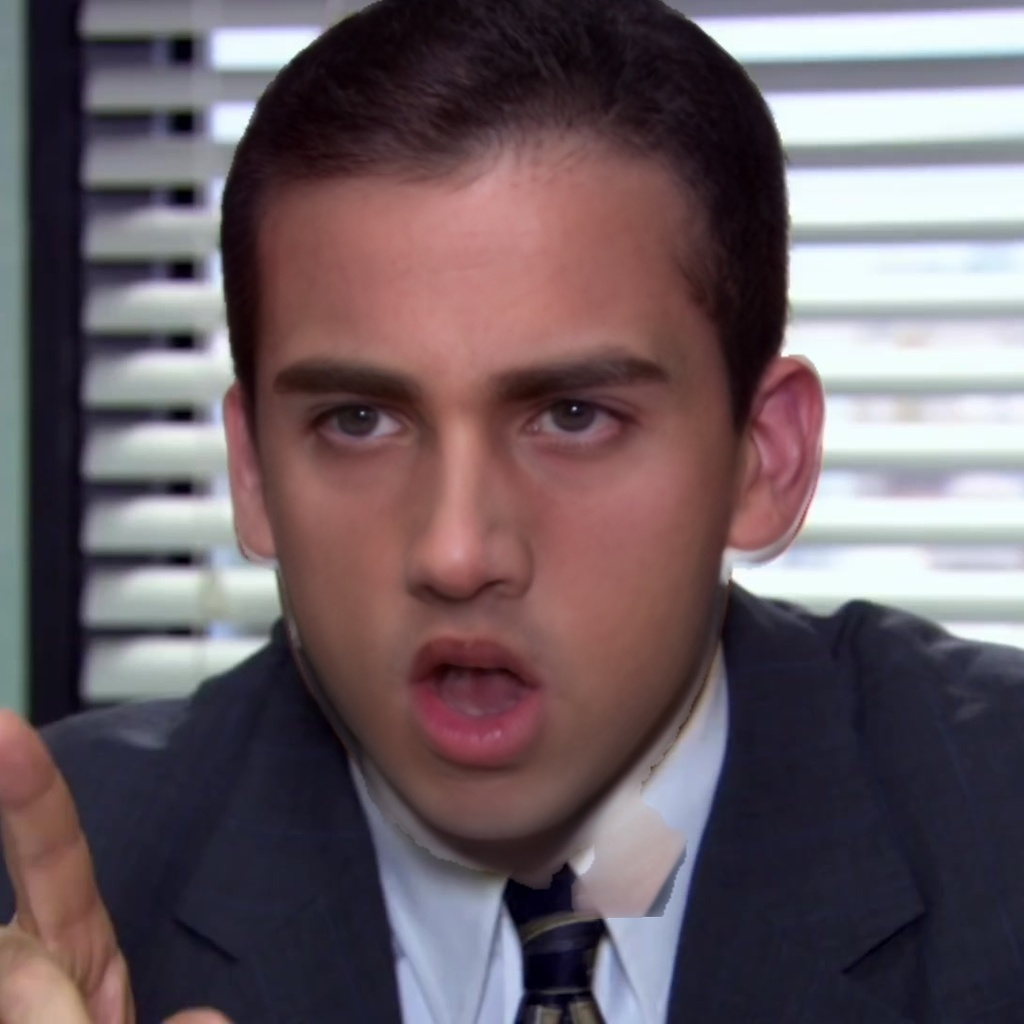
\includegraphics[width=0.24\columnwidth]{resources/images/comparison/PTI/edit_0000.jpeg}} &
\raisebox{-.42\totalheight}{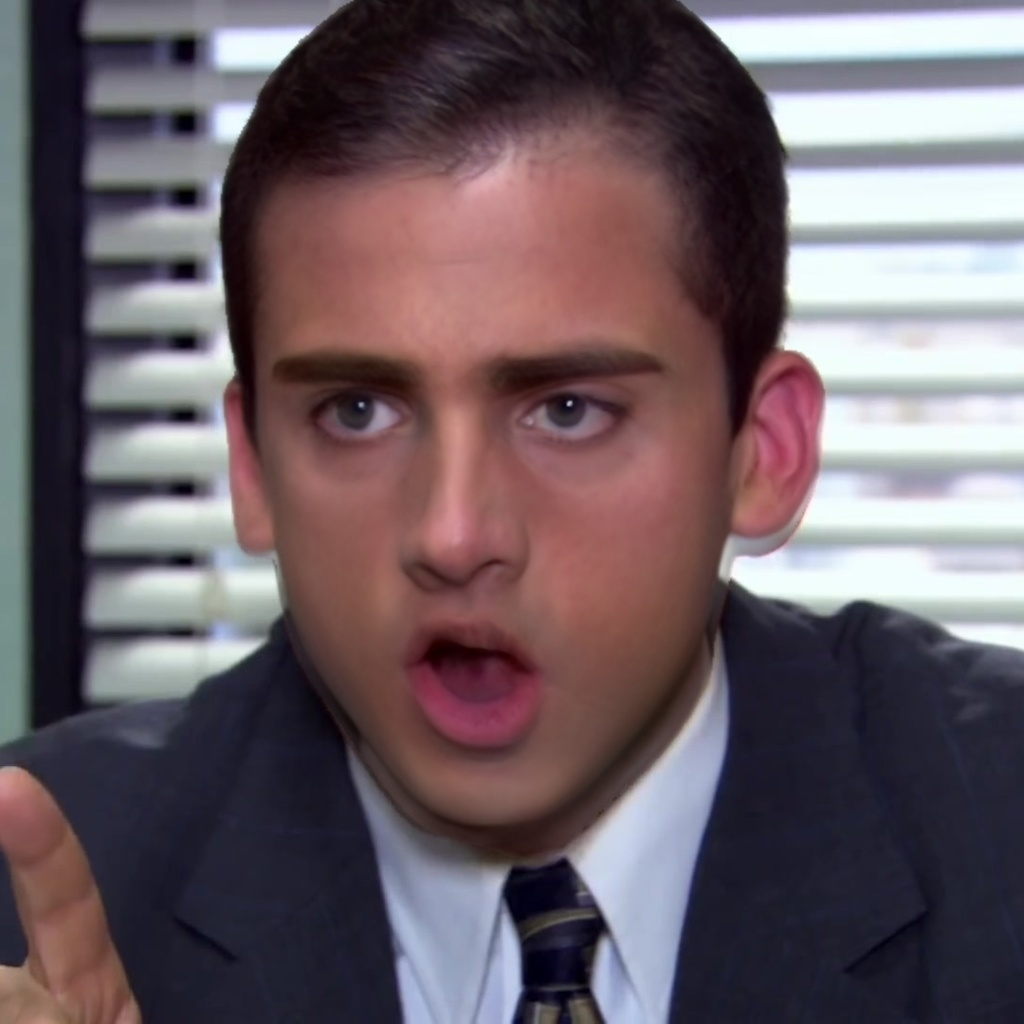
\includegraphics[width=0.24\columnwidth]{resources/images/comparison/PTI/edit_0016.jpeg}} &
\raisebox{-.42\totalheight}{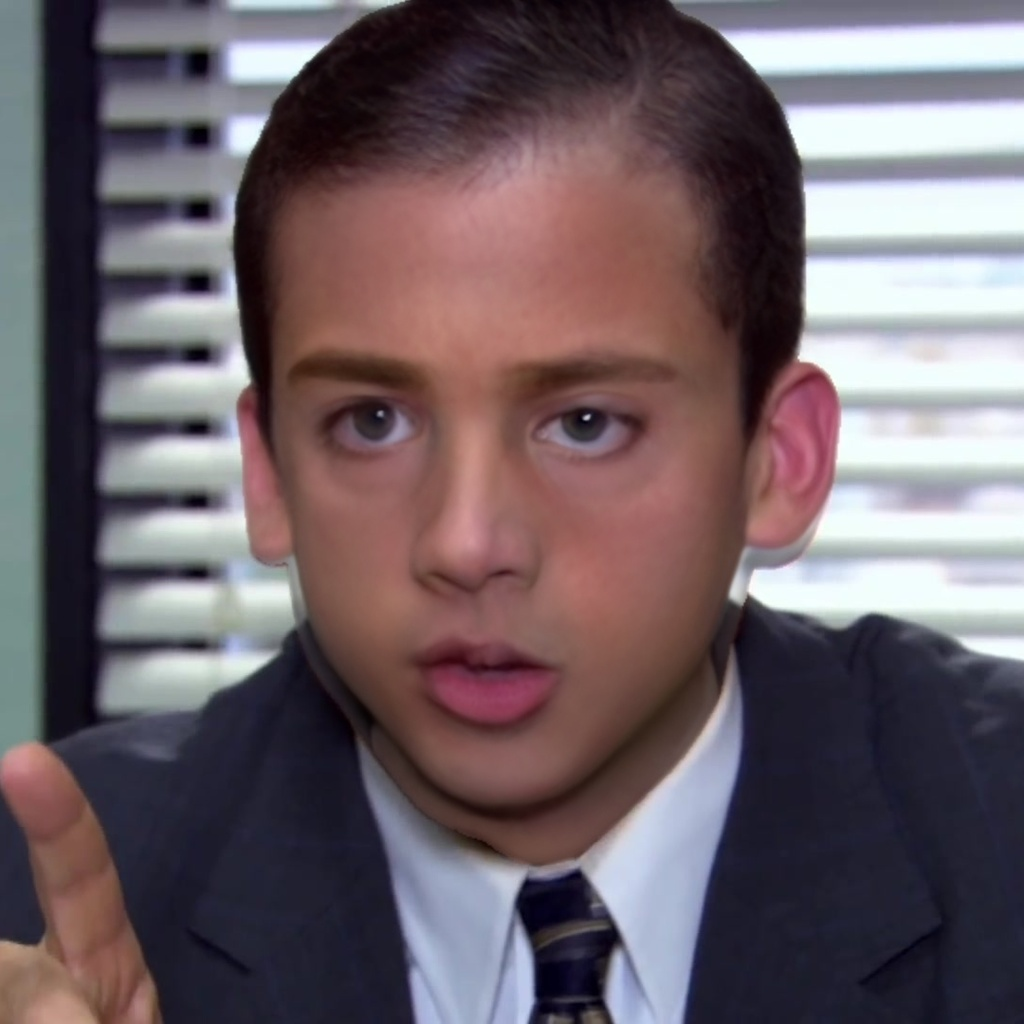
\includegraphics[width=0.24\columnwidth]{resources/images/comparison/PTI/edit_0040.jpeg}} &
\raisebox{-.42\totalheight}{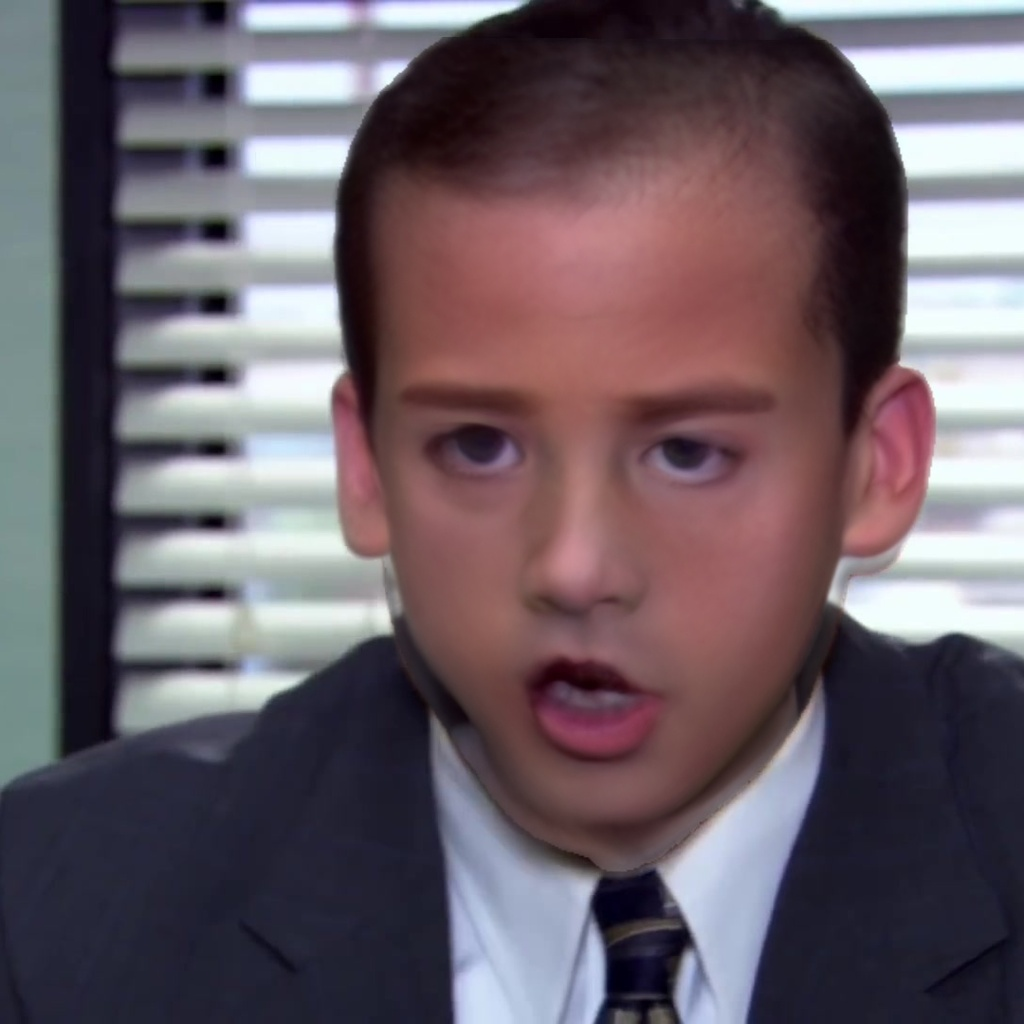
\includegraphics[width=0.24\columnwidth]{resources/images/comparison/PTI/edit_0100.jpeg}}\\
\noalign{\vskip .5mm}
\rotatebox[origin=t]{90}{Ours} &
\raisebox{-.42\totalheight}{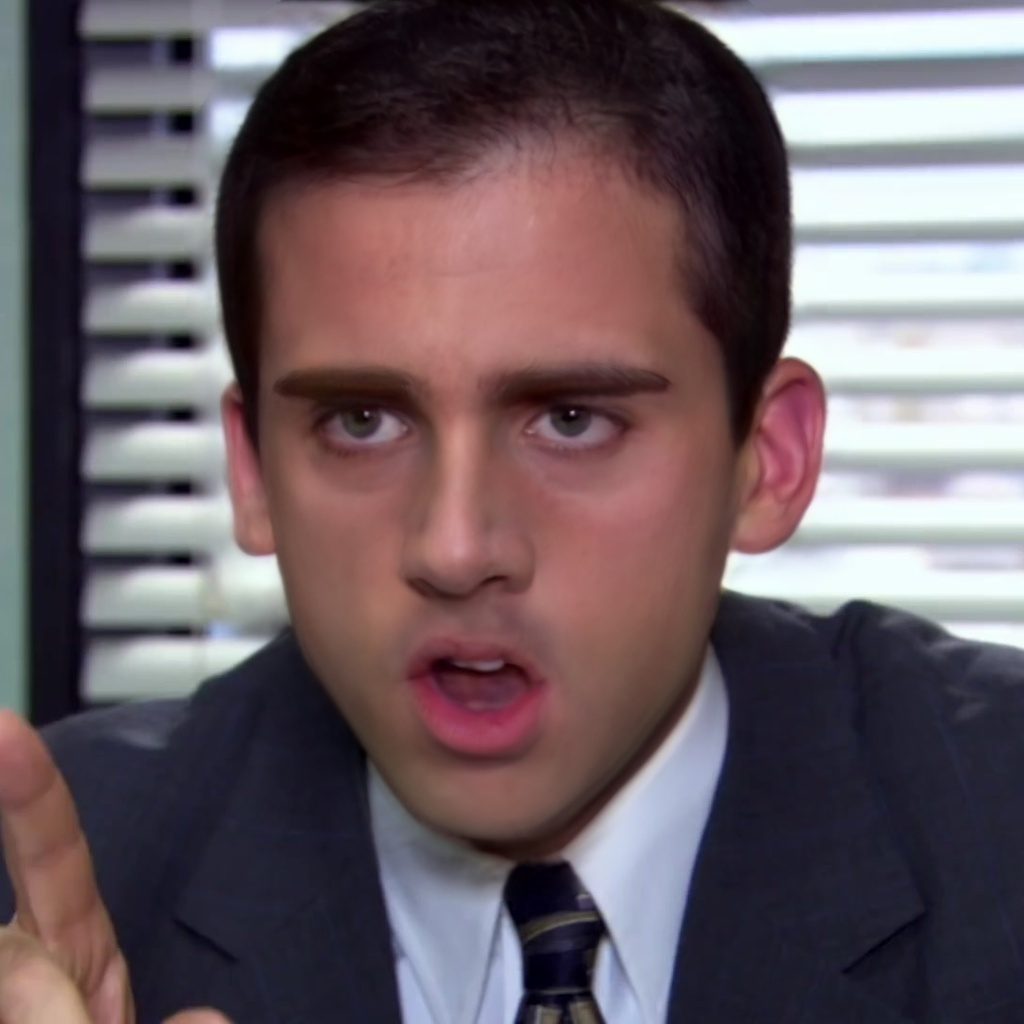
\includegraphics[width=0.24\columnwidth]{resources/images/comparison/ours/optimized_feathering_0000.jpeg}} &
\raisebox{-.42\totalheight}{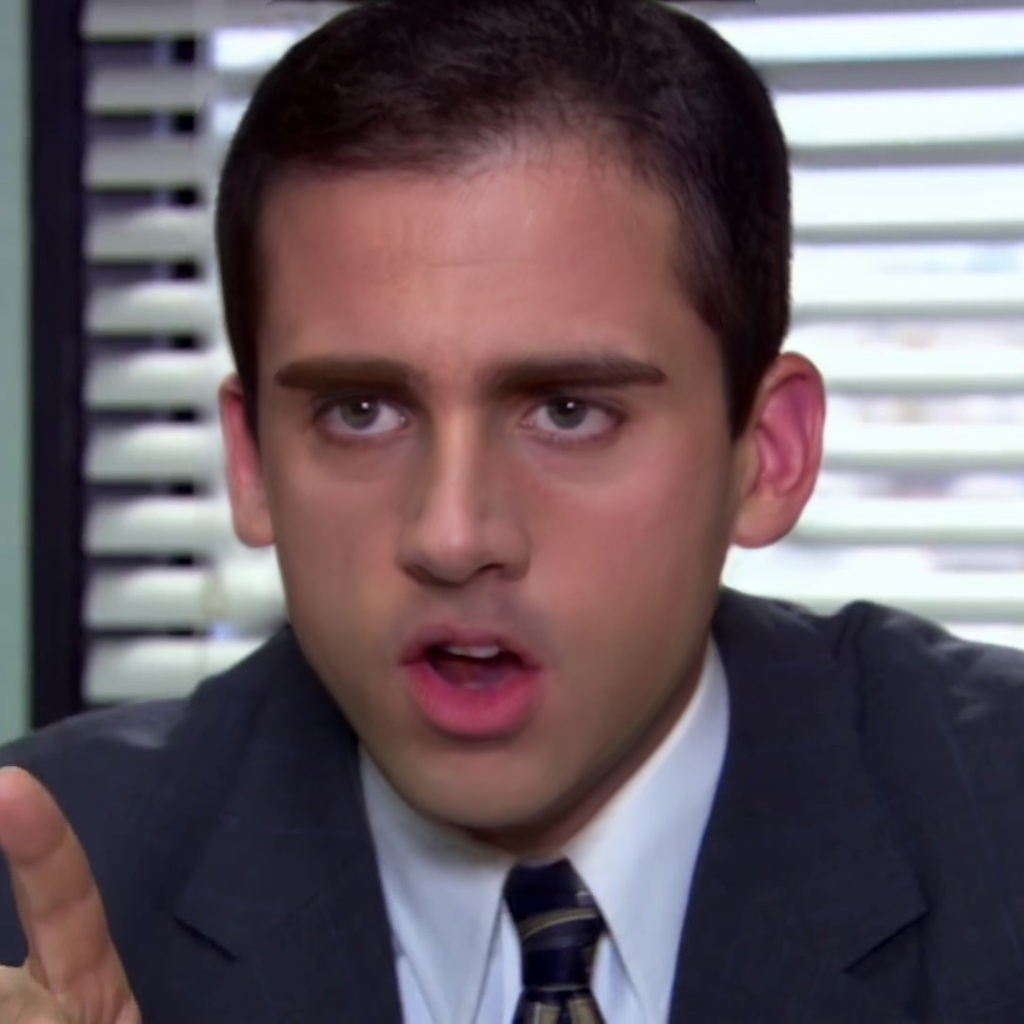
\includegraphics[width=0.24\columnwidth]{resources/images/comparison/ours/optimized_feathering_0016.jpeg}} &
\raisebox{-.42\totalheight}{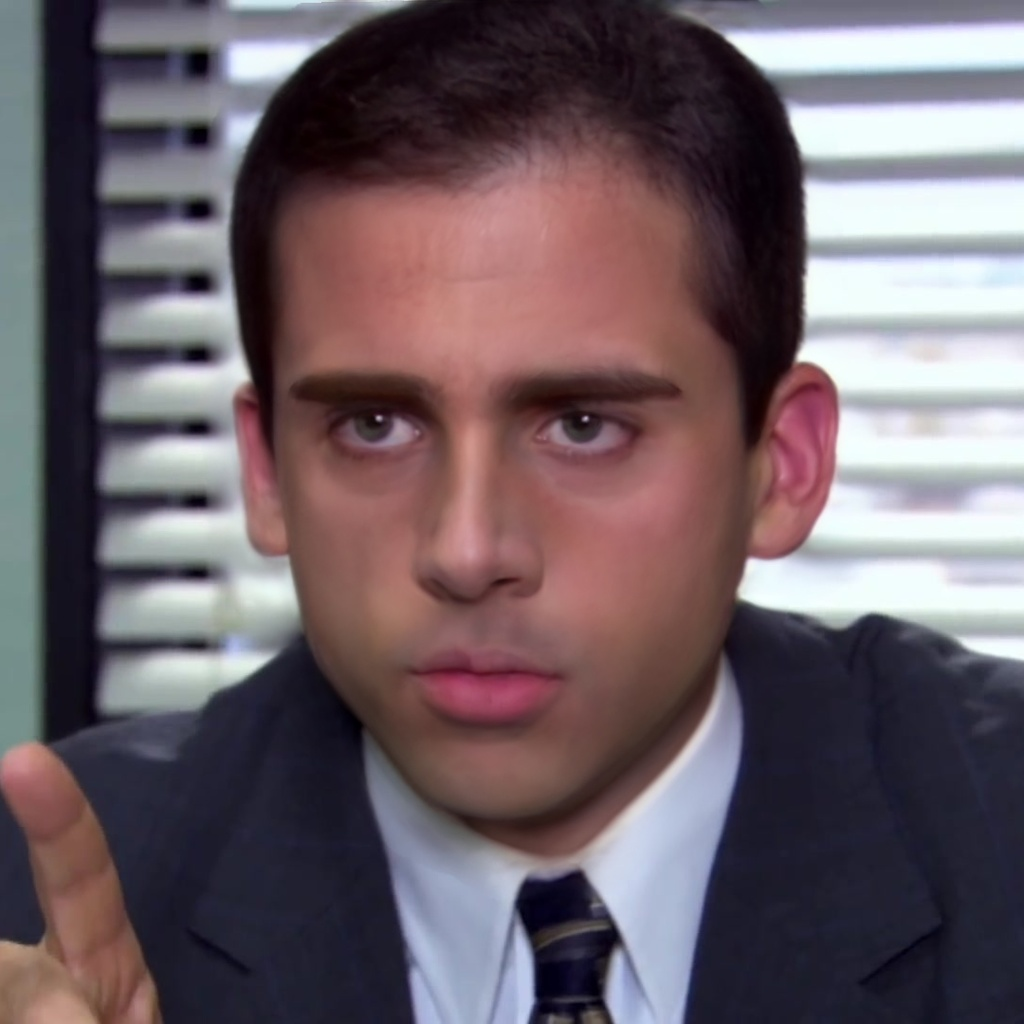
\includegraphics[width=0.24\columnwidth]{resources/images/comparison/ours/optimized_feathering_0040.jpeg}} &
\raisebox{-.42\totalheight}{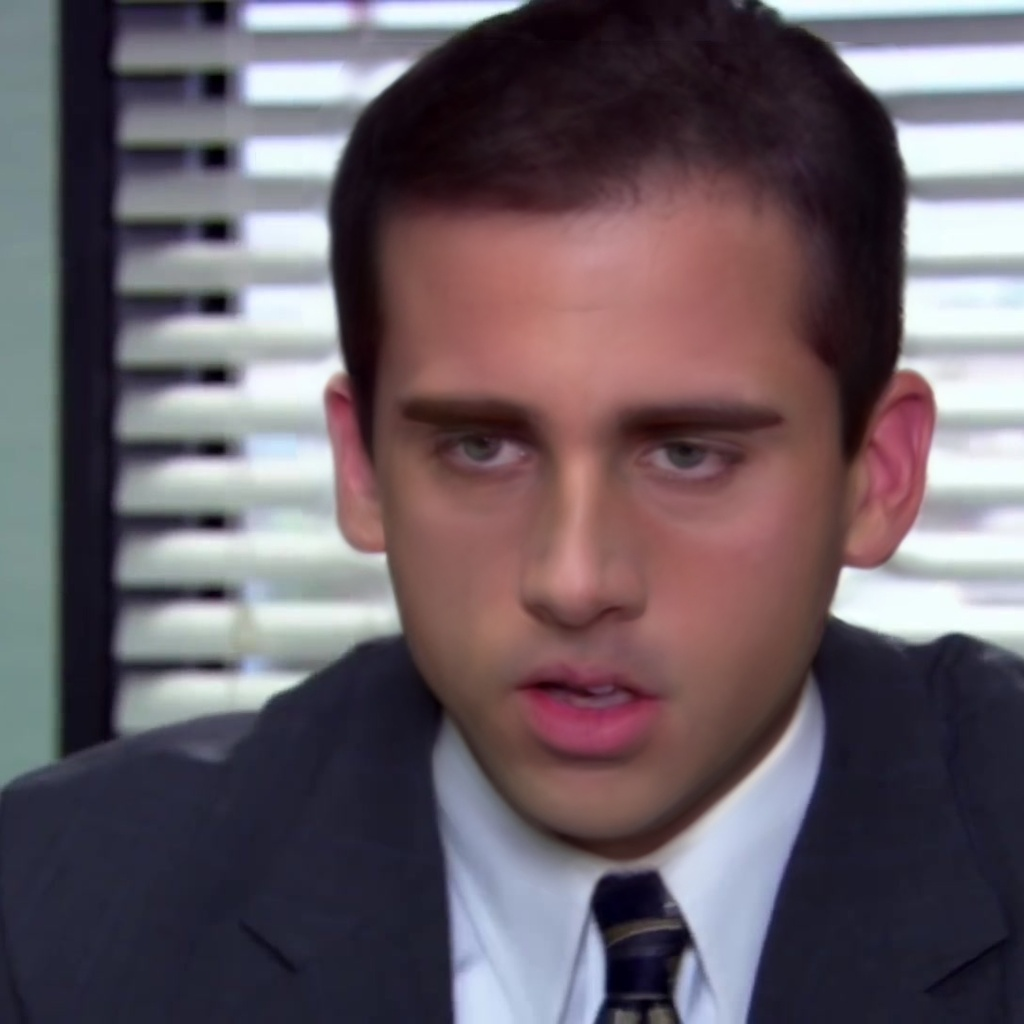
\includegraphics[width=0.24\columnwidth]{resources/images/comparison/ours/optimized_feathering_0100.jpeg}}\\
\end{tabular}
}


\caption{Visual comparison to alternative editing pipelines. Our method retains a higher degree of temporal consistency, produces realistic editing, and successfully mitigates blending-induced artifacts.}
\label{fig:comparison}
\end{figure}
